\section{{\tool} Overview}
\label{sec:overview}

\begin{figure*}[t] %[htp]
\begin{center}
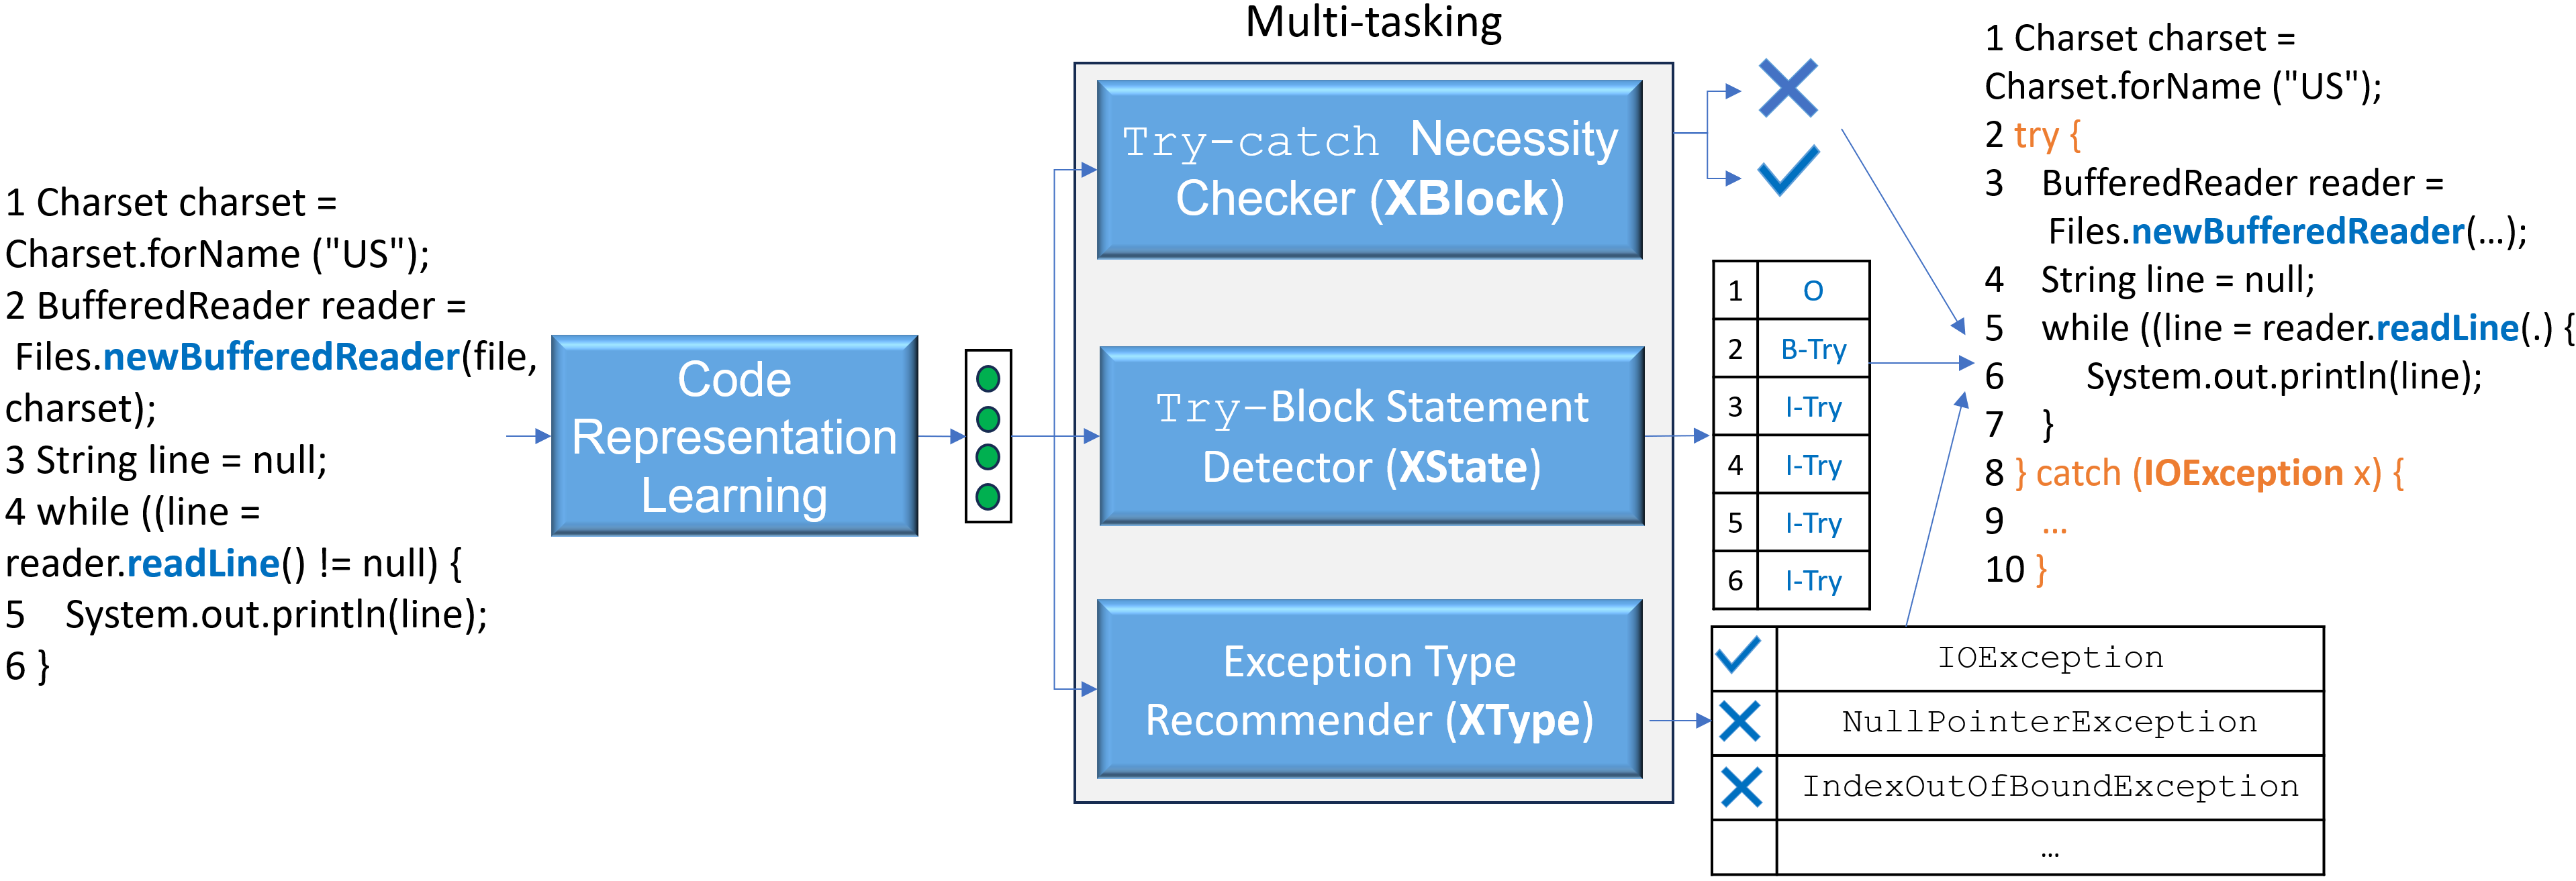
\includegraphics[width=5.7in]{overview-7.png} %5.7in, overview-6; 5: 5.65in
\vspace{-10pt}
\caption{{\tool}: Approach Overview}
\label{overview}
\end{center}
\end{figure*}

%Goals
Figure~\ref{overview} illustrates the overview of {\tool}. Generally,
{\tool} has three main components dedicated to the three tasks: for a
given (in)complete code snippet, 1) {\xblock} aims to check the
necessity of \code{try-catch} blocks, 2) {\xstate} aims to detect which
statements need to be placed within a \code{try} block, and 3) {\xtype}
aims to detect the exception types need to be caught in the
\code{catch} clause(s). We support the detection of one or multiple
\code{try-catch} blocks if any.

%training instances and prediction
During training, the code snippets with \code{try-catch} blocks in
complete code are used as the positive samples and the ones without
them as the negative ones. For a positive sample, the statements
inside the \code{try} block(s) and the exception type(s) in the
\code{catch} clause(s) are used as the labels for training. The negative
samples are labeled as not needing a \code{try-catch} block. In
prediction, {\tool} accepts as input any (in)complete code
snippet without a \code{try-catch} block, and predicts the results for
those tasks. The predicted results from {\xstate} and {\xtype} are
considered only when {\xblock} predicts {\em Yes}, i.e., a need of a
\code{try-catch} block for the given code snippet.

The input code snippet is fed into a large language model. We use
CodeBERT~\cite{codebert-emnlp20} as the code representation learning
model to produce vector representations for the (sub)tokens and
statements in the source code, as CodeBERT is capable of producing
embeddings that capture both the syntactic and semantic information.

%The input code is used as the input of a language model to act
%as the code representation learning model to produce the vector
%representations for the (sub)tokens and statements in the source
%code. We use CodeBERT~\cite{codebert-emnlp20} as it is
%capable of producing embeddings that capture both the
%syntactic and semantic information.

%The vectors are used as the inputs for three components. The
%prediction is made on the vectors that are attained by composing the
%embeddings of individual (sub)tokens into the ones for a statement and
%for a block of statements.

The vectors are used as the inputs for three components. The vectors
for the \texttt{[SEP]} tokens are used to represent the respective
statements, while the summation of the vectors for the \texttt{[SEP]} tokens at
the output layer is used for multiple statements.

First, {\xblock} is modeled as a binary classifier on deciding whether
the input code needs at least one \code{try-catch} block. Second,
inspired by the sequence chunking
techniques~\cite{sequence-chunking-aaai17} in NLP, we model the second
task, {\xstate}, as learning to tag/label each statement in the code
snippet with either \code{O} (i.e., the statement is outside of a
\code{try} block), \code{B-Try} (i.e., it is the beginning of a
\code{try} block), or \code{I-Try} (i.e., it is inside of a \code{try}
block).
%Any consecutive statements from a \code{B-try} to the last respective
%\code{I-try} are considered to belong to a \code{try-catch} block. The
%next \code{B-try} statement and its last respective \code{I-try}
%statement forms a new \code{try-catch} block and so on, if any.
During training, the statements within or outside of the
\code{try} blocks enable us to build their tags/labels.
%For prediction, the results from {\xstate} and {\xtype}
%are considered only when {\xblock} predicts {\em Yes}, i.e., a need
%of a \code{try-catch} block.

The last task, {\xtype}, is modeled as a set of binary classifiers,
each is responsible for deciding whether an exception type of interest
needs to be caught in the \code{catch} clause. A {\em Yes} outcome
indicates the need to catch a specific exception type of interest in
the set of libraries. A {\em No} outcome indicates otherwise.  During
training, the exception types for each \code{try-catch} block in a
positive sample are used as labels. During prediction, for each
predicted block from {\xstate} (starting from a statement with
\code{B-Try} to the last respective \code{I-Try}), {\xtype} uses the
embeddings for those statements to predict the corresponding exception
types. Finally, from the results in all three tasks, {\tool} forms the
final output code.

%{\bf DELETE LATER}. Given an input code snippet, we first split it by lines and concatenate them using a special token <SEP>. Then, we use the tokenizer from Pre-Trained CodeBERT to tokenize this concatenated string into sub-tokens and get the vector representation for each sub-token, as CodeBERT has been shown to have produced code representations that embed both the syntactic and semantic information. In the training phase, the input is all but the statements related to try-catch in a method body, while in the prediction phase, the input can be any code snippet that is part of a method body.

%The goal is to learn useful vector representations for a code snippet as a whole and for each statement in it so as to help the three downstream tasks. For each downstream task, we design a module , or block as we refer to it, in order to carrying out the specific learning task. The three blocks are XBlock, XState and XType. XBlock is for deciding whether the input code snippet needs any try-catch. If there are exceptions that need to be caught, XBlock outputs YES; otherwise, XBlock outputs NO. The second block is XState, where labelling technique is used to capture the statements in each try-block. In the training phase, we know whether the input contains try-block. If no try-block exists, we skip XState (and XType); In the prediction phase, we do not enter this block (and XType) if XBlock has output NO. The third block XType is for predicting which exceptions to catch for each try-block. The prediction is made on top of a vector representation of the try-block that is attained by composing individual vector representation of each statement in the try-block. In the training phase, we know which statements should be put in the same try-block as ground truth, while in prediction phase, we use the labelling results from XState to group statements into try-blocks.
%-------------------------------------

% In general, {\tool} has three main components. The first
% component, {\xblock}, aims to check if it is necessary to have a
% \code{try-catch} block for a given code snippet $C$. We extract the
% program dependence graph (PDG) from the source code using
% DeepPDA~\cite{icse23} that is capable of generating the PDG for any
% (in)complete code snippet. The PDG is used as an input for a
% Relational Graph Convolutional Network (R-GCN)~\cite{rgcn}, which acts
% as a classifier for {\xblock}. During training, we use the complete
% source code in the open-source projects in which each positive sample
% contains at least a \code{try-catch} block, and each negative sample
% does not contain any. If there are multiple consecutive blocks, we
% split them into individual ones. During prediction, {\xblock} uses the
% trained R-GCN model to predict whether the code snippet $C$ needs a
% \code{try-catch} block or not.

% In the case that the code snippet $C$ needs a \code{try-catch} block,
% the second component, {\xstate}, is aimed to detect which statements
% in $C$ that need to be placed into a \code{try-catch} block.  We model
% this task as an explanation task for {\xblock}. {\xstate} takes as
% input: 1) the PDG of the given code snippet, and 2) the trained R-GCN
% model for the \code{try-catch} necessity checker ({\xblock}), together
% with the classification result ``Yes'' from that R-GCN model of
% {\xblock}. {\xstate} leverages GNNExplainer~\cite{GNNExplainer}, a
% graph-based, Explainable AI model to decide the statements in the PDG
% that are most decisive and relevant to the reason why the code snippet
% $C$ is required to have a \code{try-catch} block. During training, in
% a positive sample, the statements in a \code{try-catch} block are
% marked as positive, and the ones outside of the block as negative. All
% the statements in a negative sample are marked as negative. During
% prediction, the output of GNNExplainer is a list of statements in
% $C$ (e.g., $S_3$, $S_4$, $S_5$) that made the R-GCN model in {\xblock}
% to decide the need of a \code{try-catch} block. We consider them as
% the statements to be in a \code{try-catch} block.

% The third component is the exception type recommender, {\xtype}.
% During training, the exception types in a \code{try-catch} block in
% the positive samples are used as the labels. During prediction,
% {\xtype} takes as input the result from GNNExplainer, which is the
% subgraph of the PDG of the given source code $C$. Another R-GCN model
% is used and acted as a classifier for all the exception
% types.
